\documentclass[notes]{beamer}

\usepackage[ngerman]{babel}
\usepackage{hyperref}
\usepackage{ragged2e}
\justifying

\title{Caelio}
\subtitle{Zwischenstand}
\author{Felix, Inga, Kilian, Lilly, Matthias}
\date{26. April 2021}
\logo
{
	
\includegraphics[width = .1\textwidth]{../../Anwendung/Icons/caelio}
}

\begin{document}
	\begin{frame}
		\titlepage
	\end{frame}
	\begin{frame}
		\centering
		ea695a4af0b181bf54dcb6b65cb71f451d3aca4a
	\end{frame}
	\begin{frame}
		\frametitle{Oberfläche}
		\thispagestyle{empty}
		\centering
		
\includegraphics[height = .5\textheight]{../../Anwendung/Icons/caelio}
	\end{frame}
	\note
	{
		\begin{itemize}
			\item Startseite: Übersicht mit allen aktuellen Werten --> User bekommt schnell und unkompliziert Überblick über aktuelle Situation 
			wieder mal Ampelsystem, das die Luftqualität anzeigen und Warnungen ausgeben soll; aber noch in Arbeit
			\item Registerkarte Einstellungen: User soll sehen können, welche Datenbank genutzt wird, diese ggf. ändern können 
			Erklärung zu Messwerten, … erhalten; aber auch noch nicht fertig
			\item Für jeden Sensor eigenen Tab, immer nach demselben Prinzip aufgebaut: Name Sensor, Symbol von Startseite, max. Wert, min. Wert, aktueller Wert
			\item alle älteren Daten sollen eigentlich noch in Tabelle und LineChart ausgegeben bzw. dargestellt werden; ist aber auch noch in Arbeit
			\item Letzter Tab für Nerds: noch Code angeben
		\end{itemize}
	}
	\begin{frame}
		\frametitle{Implementierung}
		\framesubtitle{Klassenbeziehungen}
		\begin{figure}
			\centering
			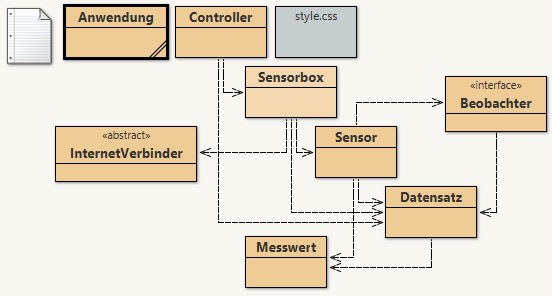
\includegraphics[width = .75\textwidth]{Abbildungen/klassenbeziehungen}
			\caption{Klassenbeziehungen des Projekts}
		\end{figure}
	\end{frame}
	\begin{frame}
		\frametitle{Implementierung}
		\framesubtitle{Klassendiagramm}
		\begin{figure}
			\centering
			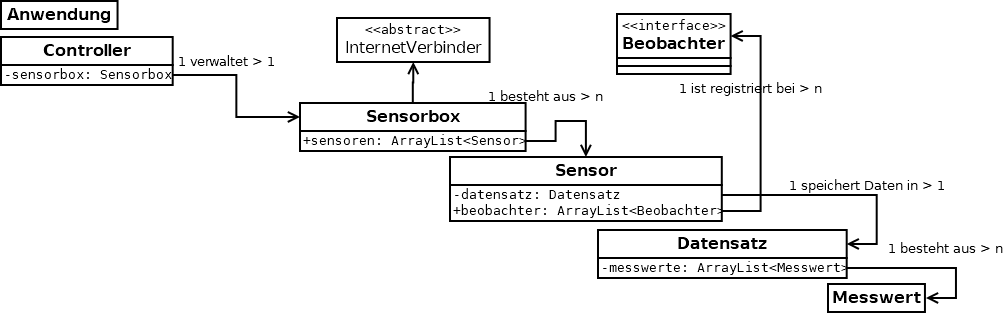
\includegraphics[width = \textwidth]{Abbildungen/klassendiagramm}
			\caption{Klassendiagramm des Projekts}
		\end{figure}
	\end{frame}
	\note
	{
		\begin{itemize}
			\item Anwendung: Starten der Anwendung.
			\item Controller: Kommunikation mit der Oberfläche.
			\item Sensorbox: Eine Sensorbox mit Sensoren mit Messwerten, die in einem Datensatz organisiert sind.
			\item Messungen werden an Beobachter weitergegeben.
		\end{itemize}
	}
	\begin{frame}
		\frametitle{Einschätzung}
		\framesubtitle{Was lief schlecht?}
		\begin{itemize}
			\item Oberfläche $\leftarrow$ Limitation auf eine Person gleichzeitig
			\item GitHub $\leftarrow$ Versionsprobleme
		\end{itemize}
	\end{frame}
	\note
	{
		\begin{itemize}
			\item Arbeit an der Oberfläche war unglaublich nervtötend und langwierig, weil immer nur eine Person daran arbeiten konnte
			\item Außerdem nervig: Problem bei GitHub, dass man immer etwas runtergeladen, verändert und dann wieder hochgeladen hat und währenddessen andere dann mit einer veralteten Version gearbeitet haben
		\end{itemize}
	}
	\begin{frame}
		\frametitle{Einschätzung}
		\framesubtitle{Was lief nicht optimal?}
		\begin{itemize}
			\item Projektboard $\leftarrow$ Unübersichtlichkeit, jedoch gute Verständigung und Planung möglich
			\item GitHub $\leftarrow$ Unübersichtlichkeit
		\end{itemize}
	\end{frame}
	\note
	{
		\begin{itemize}
			\item Arbeit mit GitHub (Projektboard) $\rightarrow$ grundsätzlich gute Verständigung und Planung möglich, jedoch wird es schnell unübersichtlich, wenn man mal vergisst dort etwas zu verschieben oder zu ergänzen - yup, sehr unübersichtlich
			\item Vlt GitHub generell sehr unübersichtlich
		\end{itemize}
	}
	\begin{frame}
		\frametitle{Einschätzung}
		\framesubtitle{Was lief gut?}
		\begin{itemize}
			\item Scrum meetings
			\item Aufteilen der Arbeit
			\item gegenseitiges Helfen
			\item Projektarbeit $\leftarrow$ Eindruck von möglichem Beruf
			\item \textbf{hat Spaß gemacht}
		\end{itemize}
	\end{frame}
	\note
	{
		\begin{itemize}
			\item Scrum meetings, Arbeit aufteilen, sich gegenseitig helfen, bla
			\item Insgesamt Projektarbeit extrem hilfreich um mal zu sehen wie ein Job in diesem Bereich so aussehen könnte; sehr interessant, hat Spaß gemacht
		\end{itemize}
	}
	\begin{frame}
		\frametitle{Organisation}
		\framesubtitle{Projektboard}
		\begin{itemize}
			\item Scrum
			\item Organisieren und Überblick
		\end{itemize}
	\end{frame}
	\note
	{
		
		\begin{itemize}
			\item Einteilung nach Scrum (Userstories, Sprints, To Do, In Progress, Dauerhaft in Progress, Done)
			\item genutzt um uns zu organisieren und den Überblick über Tasks usw. zu behalten
		\end{itemize}
	}
	\begin{frame}
		\frametitle{Organisation}
		\framesubtitle{Dauerhaft in Progress}
		\begin{itemize}
			\item weitere Ideen
			\item Testen
		\end{itemize}
	\end{frame}
	\note
	{
		\begin{itemize}
			\item weiter Ideen sammeln und Userstories verfassen
			\item Testen, damit die App problemlos und fehlerfrei funktioniert
		\end{itemize}
	}
	\begin{frame}
		\frametitle{Organisation}
		\framesubtitle{Wie haben wir unsere Sprints organisiert?}
		\begin{itemize}
			\item Daily Scrum
			\item Aufteilung von Tasks
			\item Deadlines
			\item Meetings bei Problemen und Fragen
		\end{itemize}
	\end{frame}
	\note
	{
		
		\framesubtitle{Wie haben wir unsere Sprints organisiert?}
		\begin{itemize}
			\item Daily Scrum
			\item Tasks für jeden
			\item Deadlines
			\item bei Problemen und Fragen Meetings
		\end{itemize}
	}
	\begin{frame}
		\frametitle{Organisation}
		\framesubtitle{Ideen für Zukunft des Projekts}
		\begin{itemize}
			\item Datenschutz
		\end{itemize}
	\end{frame}
	\note
	{
		\begin{quote}
			Ich möchte als Datenschützer wissen, unter welcher Lizenz das Programm steht, was für Daten die App verwendet, auf welche Daten die App zugriff haben will/hat und wie diese verwaltet werden
		\end{quote}
		$\rightarrow$ Ich als Entwickler möchte für Datenschutz in meiner App sorgen/diesen verbessern
	}
	\begin{frame}
		\thispagestyle{empty}
		\centering
		
\includegraphics[height = .5\textheight]{../../Anwendung/Icons/caelio}
		\url{https://github.com/HelgaStreithuhn/caelio}
	\end{frame}
\end{document}